\chapter{Аналитический раздел}
\label{cha:analysis}

Визуализация облаков необходима во многих обастях, от авиатренажеров до компьютерных игр.

\section{Анализ предметной области}

Визуализация облаков состоит из нескольких этапов. Для начала необходимо вычислить цвет всего неба,
для чего используется метод Переса. В данном методе цвет неба меняется в зависимосте от положения
солнца. Небо делится на несколько частей, для каждой из которых цвет вычисляется независимо
с помощию формулы \ref{eq:Perez}. На следующей итерации для вычисления цвета используются предыдущие
значения. Такой подход позволяет получить плавный переход между цветами.

\begin{equation}\label{eq:Perez}
    lv = f(\xi, \gamma) = \bigg[ 1 + a \cdot e^{\frac{b}{\cos(\xi)}} \bigg]
    \times [1 + c \cdot e^{d \cdot \gamma} + e \cdot \cos^2(\gamma)],
\end{equation}

где $lv$ - относительная яркость, $\xi$ - зенитный угол данной части неба, $\gamma$ - угол между
положением солнца и положением данного элемента.
Параметр $a$ отвечает за почернение $(a > 0)$ и осветление $(a < 0)$ области горизонта.
Коэффициент $b$ регулирует градиент яркости вблизи горизонта. Коэффициент $с$ связан с
интенсивностью солнечного ореола. Коэффициент $d$ модулирует размер области вблизи Солнца,
а параметр $e$ определяет относительную интенсивность обратного рассеивания света. Яркость
рассматриваемого небесного элемента $Lv$ может быть получена с помощью уравнения \ref{eq:Lv}.

\begin{equation}\label{eq:Lv}
    Lv = Lvz \frac{f(\xi, \gamma)}{f(0, Z)},
\end{equation}

где $Lvz$ - зенитная яркость, а $Z$ - зенитный угол солнца.

Небосвод, разделенный на области, можно увидеть на рисунке \ref{img:skydome}

\begin{figure}[H]
    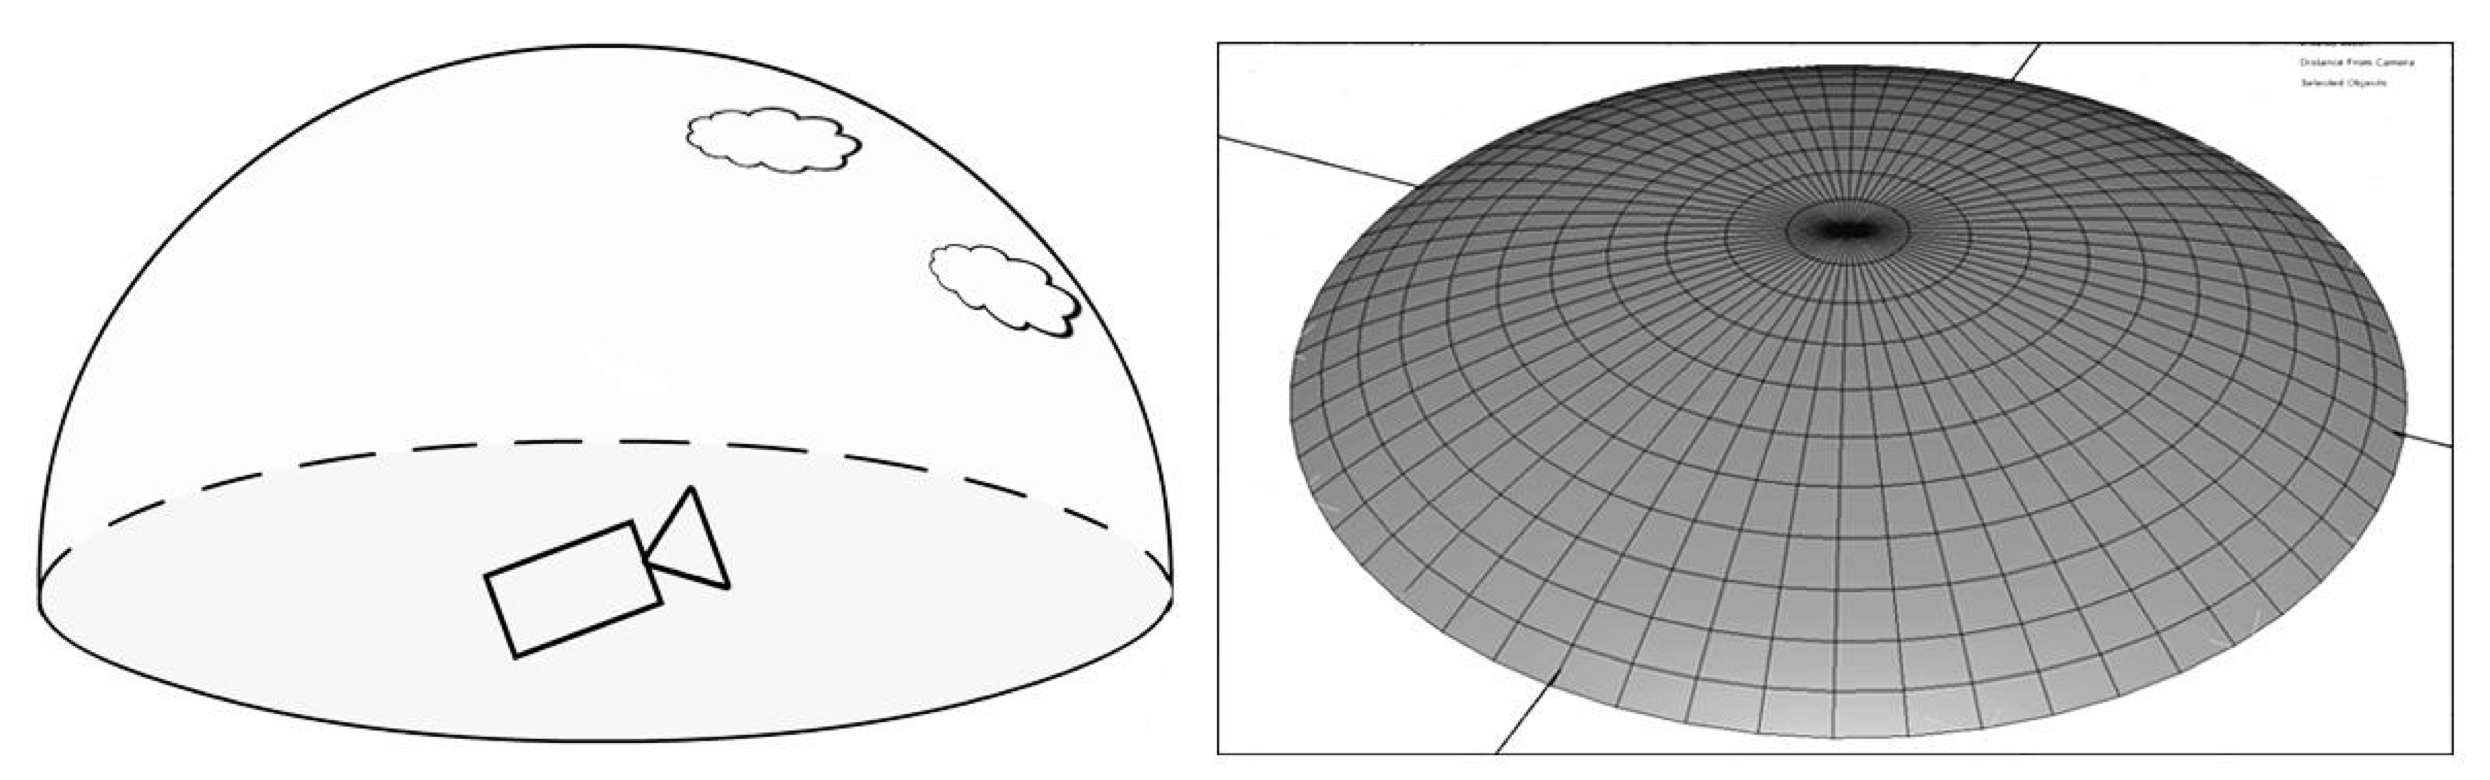
\includegraphics[scale=0.35]{img/skydome.png}
    \caption{Небосвод}
    \label{img:skydome}
\end{figure}

Participating media - это термин, используемый для описания объемов, заполненных частицами. Такими частицами могут быть крупные примеси,
такие как пыль, загрязнение, капли воды или просто молекулы.
В зависимости от своей плотности, media по-разному взаимодействуют со светом, который проходит между частиц и отскакивает от них.

\section{Обзор и анализ существующих программных систем и обоснование необходимости разработки}
